\chapter{Results}
The six stages of the workflow (see \autoref{chapter:Implementation}) are assembled into CADO, complete with GUI encapsulation. This software enables a less complicated design workflow for the user, which is described in \autoref{sec:uex}. 

In order to assess CADO's performace, several test cases are carried out. These tests, with their initial and boundary conditions, as well as the resulting optimized structures are presented in \autoref{sec:tests}.

\section{Product Overview}
\label{sec:uex}
CADO, the computer-aided design optimization tool, provides users with a turnkey solution for their design problem. CADO takes as input the geometry and boundary conditions on one hand, and simulation and surface fitting parameters on the other. The former input is given through CAD files, and the latter as numeric entries in the GUI. Using these parameters, CADO computes the optimal material distribution and reconstructs a fully CAD-compliant geometry from it.

In terms of user experience, CADO offers simplicity and intuitiveness. It requires no knowledge of its algorithms and implementation from the user. Provision of all parameters and files necessary for the simulation is seamlessly integrated into the GUI (see \autoref{fig:mainWindowParameters}). Once under progress, the status of the simulation can be assessed throught the progress bars, corresponding to the three major steps:
\begin{itemize}
\item Voxelization
\item Topology Optimimzation
\item Surface Fitting
\end{itemize}
Further information and the detailed description of the user interface can be found in the userguide (see \autoref{app:userGuide}). CADO itself is licensed under the open source BSD license and can be found on Github \cite{CADOGit}.


\section{Test Cases}
\label{sec:tests}
The performance of CADO is evaluated through three tests. The first case is a standard Cantilever design problem in three dimensions. The second deals with optimization of a bridge design. Finally, the third case leans more towards real-world applications, and concerns a design challenge on a jet engine bracket. Here we describe the underlying boundary conditions and the outcome of the tests.
\newpage
\subsection{Cantilever}
\label{ssec:canti}
The first test case simulates a cantilever. A cuboidal block of material is provided as the initial condition. This block is fixed at one end to a wall. The load on the cantilever is modeled as a downward force on its other end. (see \autoref{fig:cantiBC}).
\begin{figure}[H]
\begin{center}
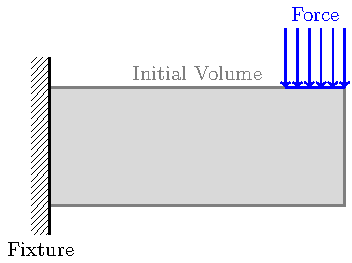
\includegraphics[scale=0.8]{Pictures/tikzCantilever/canti.pdf}
\end{center}
\caption{Boundary conditions for the test case "Cantilever".}
\label{fig:cantiBC}
\end{figure}

The cantilever is first modeled on a CAD designer (\autoref{fig:cantiCAD}). With all necessary input files and parameters, CADO produces a topology-optimized structure (\autoref{fig:cantiOPTIM}). There is a $78\%$ reduction of volume as compared to the initial configuration. The NURBS surface enclosing this volume consists of $2202$ single NURBS patches.

\begin{figure}[H]
\begin{subfigure}[t]{.45\textwidth}
\begin{center}
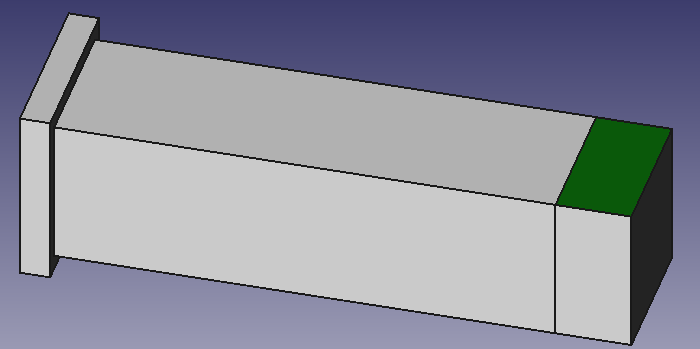
\includegraphics[width=.9\textwidth]{Pictures/Results/CantiIn.png}
\end{center}
\caption{CAD design}
\label{fig:cantiCAD}
\end{subfigure}
\begin{subfigure}[t]{.45\textwidth}
\begin{center}
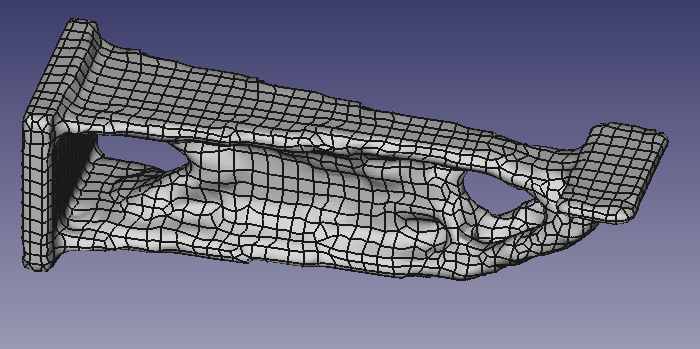
\includegraphics[width=.9\textwidth]{Pictures/Results/CantiOut.png}
\end{center}
\caption{Optimized structure}
\label{fig:cantiOPTIM}
\end{subfigure}
\caption{Test case "Cantilever"}
\end{figure}
\newpage


\subsection{Bridge}
The second test scenario simulates a bridge as a volume resting on two supports and a plane -- the intended driving plane -- in the middle of the volume. This plane is subjected to an area force that models the load of traffic as well as the bridge's self weight. The two fixtures are intentionally placed at non-symmetric positions ($a\neq b$, see \autoref{fig:bridgeBC}).
\label{ssec:bridge}
\begin{figure}[H]
\begin{center}
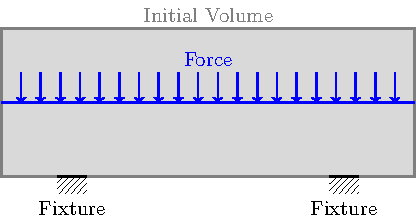
\includegraphics[scale=0.8]{Pictures/tikzBridge/bridge.pdf}
\end{center}
\caption{Boundary conditions for the test case "Bridge".}
\label{fig:bridgeBC}
\end{figure}
The bridge modeled in CAD (see \autoref{fig:bridgeCAD}) and processed through CADO. The CAD output shows a wholesome balance between intuition and efficiency -- it complies with the intuitive idea of a bridge, and also ensures minimal use of material. (see \autoref{fig:bridgeOPTIM}). The optimized structure is represented by $868$ NURBS patches, with approximately $85\%$ reduction of volume. We also observe "dents" on the surface of the driving plane.
\begin{figure}[H]
\begin{subfigure}[t]{.45\textwidth}
\begin{center}
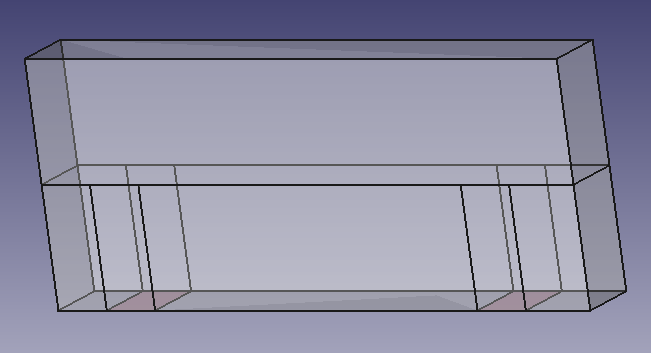
\includegraphics[width=.9\textwidth]{Pictures/Results/BridgeIn.png}
\end{center}
\caption{CAD design}
\label{fig:bridgeCAD}
\end{subfigure}
\begin{subfigure}[t]{.45\textwidth}
\begin{center}
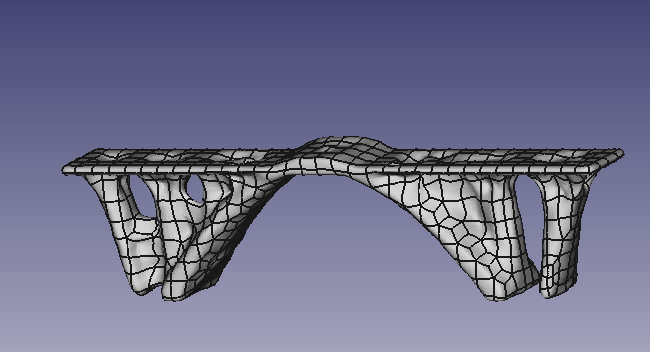
\includegraphics[width=.9\textwidth]{Pictures/Results/BridgeOut.png}
\end{center}
\caption{Optimized structure}
\label{fig:bridgeOPTIM}
\end{subfigure}
\caption{Test case "Bridge"}
\end{figure}
\newpage


\subsection{GE Jet Engine Bracket}
\label{ssec:bracket}
\begin{figure}[H]
\begin{center}
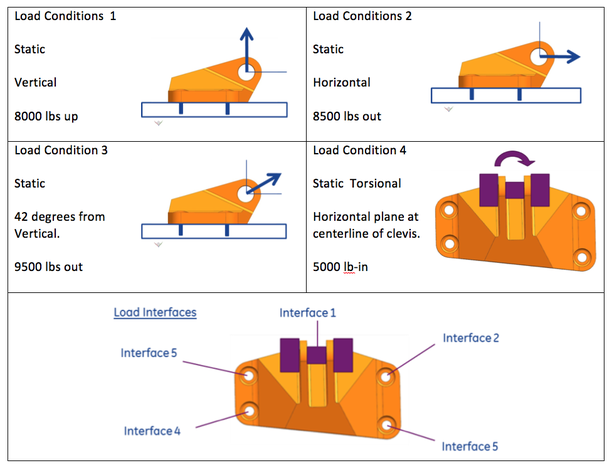
\includegraphics[scale = 0.4]{Pictures/GEbracket.png}
\end{center}
\caption{Boundary conditions and different load cases for test case "GE Bracket". Figure from \cite{GEBracket}.}
\label{fig:GEbracketBC}
\end{figure}

On the contrary to the previous two tests, the final test case resembles a real application scenario. The load conditions and the initial volume originate from a topology optimization challenge proposed by General Electric in 2013 \cite{GEBracket}. The original goal of the challenge was the optimization of a jet engine bracket, that is subjected to four different load conditions and five different non-changing regions (see \autoref{fig:GEbracketBC}).

In the following an already optimized design from \cite{GEBracketTripon} was chosen, since the scale of the scenario was too big to be handled by the topology optimizer ToPy, due to runtime and memory constraints. Therefore, the task for the last test case was only the reconstruction of the given geometry, in order to investigate the performance of the surface fitting algorithm for real-world applications. While the original design is described by $226$ faces, the reconstructed version took $3202$ NURBS patches. Additionally some topological features are lost in the region close to "Interface 1"(see \autoref{fig:GEbracketBC}).
\enlargethispage{2cm}
\begin{figure}[H]
\begin{subfigure}[t]{.45\textwidth}
\begin{center}
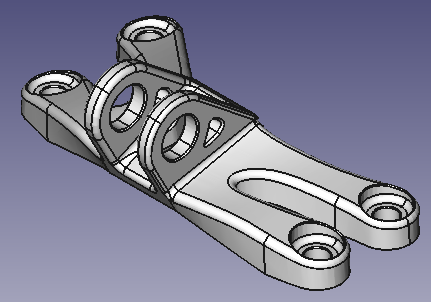
\includegraphics[width=.9\textwidth]{Pictures/Results/BracketIn.png}
\end{center}
\caption{CAD design. Initial geometry is already an optimized design from \cite{GEBracketTripon}.}
\label{fig:GEbracketCAD}
\end{subfigure}
\begin{subfigure}[t]{.45\textwidth}
\begin{center}
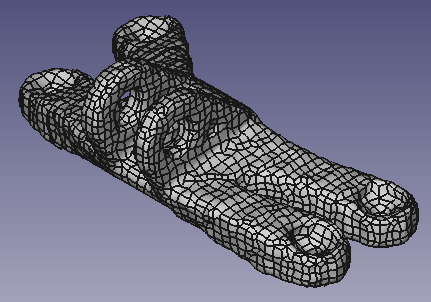
\includegraphics[width=.9\textwidth]{Pictures/Results/BracketOut.png}
\end{center}
\caption{Reconstructed structure}
\label{fig:GEbracketOPTIM}
\end{subfigure}
\caption{Test case "GE Bracket"}
\end{figure}

